\documentclass{article}
\usepackage[utf8]{inputenc}
\usepackage{amsmath,amssymb,amsthm}
\usepackage{graphicx}

\newtheorem{claim}{Claim}
\newtheorem{lemma}{Lemma}
\newcommand{\half}{\tfrac{1}{2}}
\newcommand{\tr}{\mathop{\text{tr}}}
\newcommand{\E}{\mathbb{E}}
\renewcommand{\L}{\mathcal{L}}
\newcommand{\N}{\mathcal{N}}
\newcommand{\R}{\mathbf{R}}

\title{Good Step Size Policies Adjust Often, Look Ahead, and Don't Try to Minimize the Objective Function}
\author{ali, ying, moshe, tamas, sushant, rina, shankar, alan}
\date{August 2016}

\begin{document}

\maketitle

\section{Introduction}

In deterministic numerical optimization, where search directions depend only on the current iterate, line searches offer a way to pick step sizes that guarantee fast convergence. In the stochastic setting, where search directions are random functions of the current iterate, relatively little seems to be know about line searches. What is the ideal step size in each iteration? Should one strive to approximate the true mean function and conduct line searches on it? Or is it better to perform a line search on the stochastic instances of this function? Is a line search even a good idea?

We analyze line searches in the context of minimizing quadratic cost functions with stochastic gradient descent. {\it Be upfront that we don't actually offer a practical algorithm. We're trying to understand why our experiments didn't work.} 

Surprises abound:
\begin{itemize}
    \item  Even if one had access to the true mean function, and one isn't charged for the line search at each iteration, a line search on the mean function would cause slower convergence than a fixed step size.
    \item SGD converges much faster with a line search on the random realizations of the function than on the mean function, despite the fact that the mean function is the objective of interest.
    \item One can represent the search for the optimal line search as a Markov Decision Process, and explicitly compute in closed form the optimal function on which to conduct the line search. This function turns out to be neither of the aforementioned candidates, but rather, a deterministic function whose Hessian is the inverse of that of the mean function's. 
    \item The rate of convergence of SGD with this optimal line search has nearly the same asymptotic rate  as Newton's method with exact Hessian and stochastic gradient. This rate depends only logarithmically on the condition number of the problem. In a deterministic setting, it would be unfathomable for gradient descent with any scalar step size to achieve such a rate. But in the the stochastic setting, scalar step sizes can steer the expected direction of the gradient, and serve as preconditioners.
\end{itemize}


Here are the detail of the stochastic quadratic model we investigate: The value and gradients of a random quadratic on $\R^d$ are observed:
\begin{equation}\label{eq:stoch-model}
f_a(x) = \half \left[a^\top (x-x^*)\right]^2, \qquad \nabla f_a(x) = aa^\top (x-x^*),
\end{equation}
where $a$ is a random vector drawn from a zero-mean Gaussian with covariance matrix $A$. The goal is to find $x^*$, the minimizer of the mean function,
\begin{equation}\label{eq:mean-model}
 \E_a f_a(x) = \half (x-x^*)^\top A (x-x^*).
\end{equation}
This model amounts to an overdetermined least squares problem where the independent variables are Gaussian vectors $a$ and the dependent variable is $a^\top x^*$,  a deterministic function of the dependent variables.

Stochastic gradient descent repeatedly applies the map
\begin{equation}
x_{t+1} \leftarrow x_t - \gamma \nabla f_a(x_t), \label{eq:sgd}
\end{equation}
where the direction $\nabla f_a$ is stochastic.

Our concern is to find a good choice of the step size $\gamma$ at each iteration that causes $\E_a f_a(x_t)$ to shrink quickly as a function of $t$. In practice, the cost of computing $\gamma$ is an important consideration, but because we seek to characterize the behavior of SGD under an ideal $\gamma$, we allow ourselves significant leeway in the choice of algorithms for computing $\gamma$.

Consider two plausible strategies for picking $\gamma$. One is to minimize $\E f$ along the search direction:
$$\gamma_{mean}(x,a) \equiv \arg\min_\gamma\; \E_b f_b(x-\gamma \nabla f_a(x)).$$
where the direction $\nabla f_a$ is stochastic, but the expected value of the objective function is available. In the machine learning setting, the gradient would be computed on a mini-batch, and the line search would be conducted on the full dataset. This is obviously not a practical strategy, but one that others have instinctively sought to approximate.

Another strategy is to minimize $f_a$ along the search direction:
$$\gamma_{sgd}(x,a) \equiv \arg\min_\gamma f_a(x-\gamma \nabla f_a(x)).$$
Here, both the direction $\nabla f_a$ and the value of the objective function are stochastic. In the machine learning setting, the line search and the stochastic gradient would be computed on the same batch.

More broadly, we're interested in a function $\L$ so that the line search
$$\gamma_\L(x,a) \equiv \arg\min_\gamma \L(x-\gamma \nabla f_a(x))$$
causes $\E_a f_a(x_T)$ to be small at the ultimate iterate $T$.

\begin{figure}
    \centering
    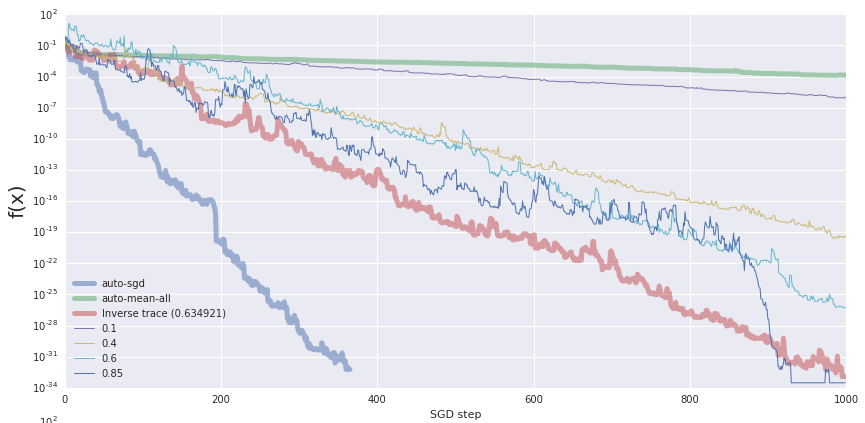
\includegraphics[width=12cm]{cond=20-dim=3}
    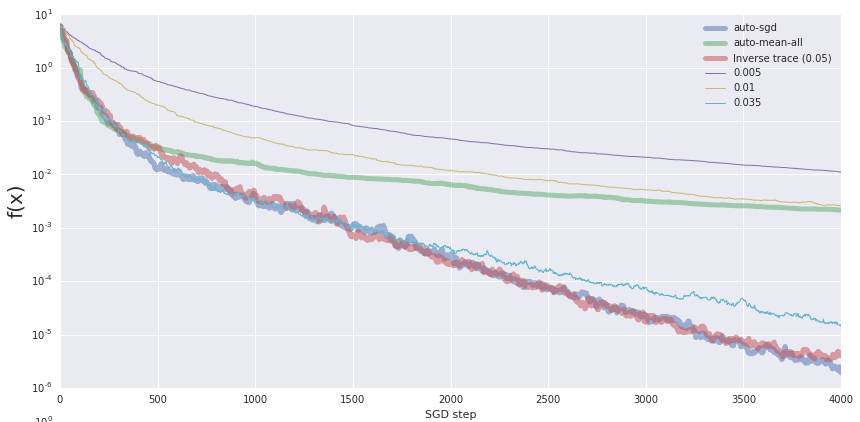
\includegraphics[width=12cm]{cond=1e6-dim=40}
    \caption{A line search over the mean function ({\tt auto-mean-all}), which is the objective of interest, causes stochastic gradient descent to converge very slowly. SGD with a fixed step size (including {\tt inverse-trace}, an automatically computed fixed step-size that maximizes the greedy convergence rate) converges faster. A line search on the stochastic function ({\tt auto-sgd}) converges even faster. Experiments are on a stochastic quadratic described by Equations (\ref{eq:stoch-model}) and (\ref{eq:mean-model}). In the top panel, the covariance $A$ is $3\times 3$ matrix with condition number 100. In the bottom panel, $A$ is $40\times 40$ with condition number $10^6$. The larger dimensionality causes the minimizer of the stochastic function to converge to the automatically computed fixed step size.}
    \label{fig:emp}
\end{figure}

The empirical observation that prompted this note is this: With step size size $\gamma_{mean}$, the objective $\E_a f_a(x_t)$ decays more slowly over $t$ than with step size $\gamma_{sgd}$. See Figure \ref{fig:emp}. This is surprising because $\gamma_{mean}$ was explicitly chosen to minimize $\E_a f_a$, the very objective we wanted to minimize. Even more surprisingly, fixed step sizes also outperform $\gamma_{mean}$.

Furthermore, there is a step size that outperforms even $\gamma_{sgd}$. The optimal step size policy for the quadratic model is a line search over a deterministic function whose Hessian is the inverse of that of $\E f$. This function behavior in some ways in the exact opposite way of $\E f$. The reason $\gamma_{sgd}$ outperforms $\gamma_{mean}$ is that it is a better approximation to this optimal step sizing rule. See Figures \ref{fig:faster} for comparisons.

\begin{figure}
    \centering
    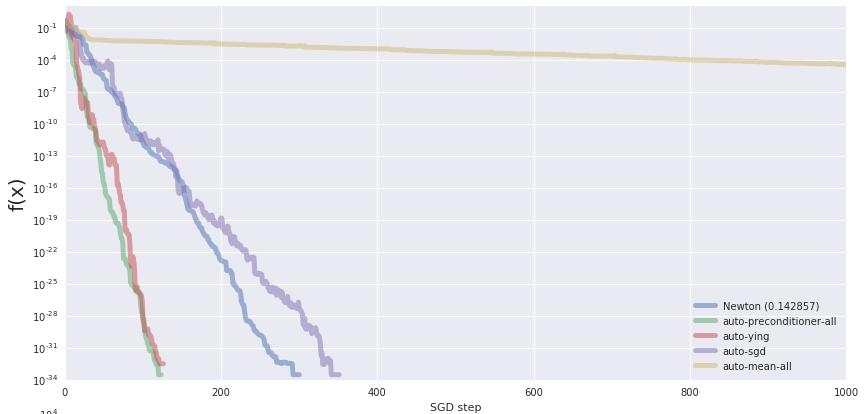
\includegraphics[width=12cm]{faster-cond=20-dim=3}
    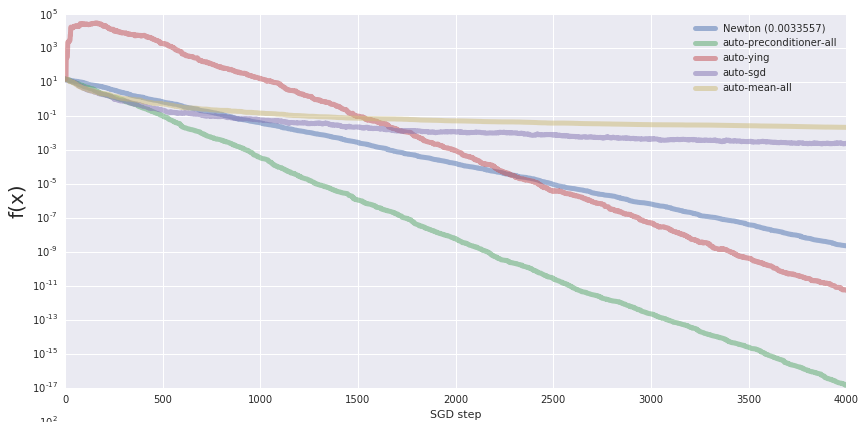
\includegraphics[width=12cm]{faster-cond=1e6-dim=40}
    \caption{An optimal line search ({\tt auto-ying}) causes stochastic gradient descent to converge nearly as faster as second order methods. The two second order methods in question are Newton step that rely on the exact Hessian and on the stochastic direction ({\tt Newton}), and a preconditioned version of the problem, which amounts to Newton steps, but with the step sizes chosen by minimizing the stochastic function ({\tt auto-preconditioner-all}). The top panel is the three-dimensional problem with condition number 20. The bottom panel is the 40-dimensional problem with condition number $10^6$.}
    \label{fig:faster}
\end{figure}

\section{Optimal Step Sizes For Random Quadratics}

Ultimately, the quantity one cares about is not the rate of decay of $\E_a f_a$ from one iteration to the next, but rather, the value of the function at the last iterate, $\E_a f_a(x_T)$.  Finding the step sizing rule that minimizes this quantity requires planning ahead. Iterates with identical objective value can converge to $x^*$ at dramatically different rates, even on the foregoing quadratic model. So as early as $x_1$, a bad step size can land $x_2$ into a region where progress is slow thereafter.

At each iteration, choose $\gamma$ to minimize the value of the ultimate iterate, $\E f_a(x_T)$, and assume that subsequent step sizes are similarly chosen. The expectation here is over the entire sequence of $a$'s leading to $x_T$. Let $\L_t(x_t)$ denote the objective value $\E_a f_a(x_T)$ starting from $x_t$ and assuming $\gamma$ is chosen optimally from time $t$ onward:
\begin{align}
\L_t(x_t) &= \E_a \min_\gamma \label{eq:Lt} \L_{t+1}\left(x_t - \gamma \nabla f_a(x_t)\right) \\
\L_T(x_T) &= \E_a f_a(x_T).
\end{align}
$\L_t(x_t)$ is large when the gradients at $x_t$  are distributed so that no sequence of subsequent step sizes can ensure $\E_a f_a(x_T)$ is small. The choice of $\gamma$ in the definition of $\L$ explicitly tries to avoid such bad regions.

Accordingly, the best step size at time $t$ is given by:
$$\gamma_t(x_t,a) = \arg\min_\gamma\; \L_{t+1}(x_t - \gamma \nabla f_a(x_t)).$$
At $T-1$, the optimal step size is then just a line search on the mean function. But things are very different earlier on.


\begin{claim}\label{claim:main}
 With $f_a(x) = \half \left[a^\top (x-x^*)\right]^2$, and $a \in \R^d$ a stochastic sub-gaussian vector, $\L_1(x_1)$ is quadratic in $x_1$. Furthermore, with $d$ large, as $T\to \infty$, there exists a sequence of positive scalars $c_1\ldots c_T$ so that 
 $$\L_1(x_1) \approx c_T (x_1-x^*)^\top A^{-1} (x_t-x^*).$$
 
 The $\approx$ needs more work. It is only true if $T$ and $d$ are  balanced.
\end{claim}
Thus the optimal line search is on $\L_1(x) \propto \half (x-x^*)^\top A^{-1} (x-x^*)$, and not on $\E_a f_a(x) = \half (x-x^*)^\top A (x-x^*)$.

We'll need the following lemma to prove the claim:

\begin{lemma}\label{lemma:inverse}
Let $a\in \R^n$ be a vector with positive components. Consider the iterations
\[
x_i^{(t+1)} \leftarrow x_i^{(t)} - a_i \left[x_i^{(t)}\right]^2/\sum_i a_i x_i^{(t)},
\]
and the function 
\[
\ell(x) \equiv \frac{\max_i x_i a_i}{\min_i x_i a_i}-1.
\]
If the initial iterate $x^{(0)} \in \R^n$ has positive components, subsequent iterates satisfy
\[
\ell(x^{(t)}) \leq \ell(x^{(0)}) \left(1-\frac{1}{n-1}\right)^t.
\]
\end{lemma}

The Lyapunov function $\ell$ measures the deviation between $x_i$ and $1/a_i$. It attains its minimum when $x_i = \frac{c}{a_i}$ for any constant $c$. The lemma therefore implies $x_i^{(t)} \to \frac{c_t}{a_i}$ as $t\to\infty$ for some sequence of scalars $c_t$. 
 
\begin{proof}[Proof of Claim \ref{claim:main}]
To simplify notiation, define $v_t\equiv x_t-x^*$, so that $\nabla f_a(x_t) = aa^\top v_t$ and $\E_a f_a(x_t) = \half \|v_t\|_A^2$.

Assume the base case that $\L_{t+1}(x_{t+1})$ is a quadratic $\half \|v_{t+1}\|_{B_{t+1}}^2$ for some symmetric matrix $B_{t+1}$. This is true for $\L_T$ with $B_T=A$. Then
\begin{align}
\L_t(v) &= \E_a \min_\gamma \half \|v-\gamma aa^\top v\|_{B_{t+1}}^2 \\
&= \E_a \min_\gamma \half \|v\|_{B_{t+1}}^2 - \gamma  (a^\top v)(a^\top B_{t+1} v) +  \half \gamma^2  (a^\top v)^2 (a^\top B_{t+1} a).
\end{align}
Plugging back the minimizer $\gamma_t^* = \frac{a^\top B_{t+1} v}{(a^\top v)(a^\top B_{t+1} a)}$ gives
$$\L_t(v) = \half \|v\|_{B_{t+1}}^2 - \half \E_a \frac{(a^\top B_{t+1} v)^2}{a^\top B_{t+1} a}.$$
By Rina and Ying, the denominator in the expectation concentrates, yielding
\begin{align}
\L_t(v) &\approx \half \|v\|_{B_{t+1}}^2 - \frac{v^\top B_{t+1} A B_{t+1} v }{2\tr B_{t+1} A} \\
&= \half v^\top \left(B_{t+1} -   \frac{B_{t+1} A B_{t+1}}{\tr B_{t+1} A} \right) v,
\end{align}
or as a recurrence,
\begin{align}
B_T &= A \\
B_t &= B_{t+1} - \frac{B_{t+1} A B_{t+1}}{\tr B_{t+1} A} \label{eq:recurrence}\\
\L_t(v) &= \half \|v\|_{B_t}^2.
\end{align}

Now solve the recurrence assuming $T\to\infty$. Let $A=PD_AP^\top$ be the eigendecomposition of $A$. Then the eigendecomposition of $B_t$ takes the form $PD_{B_t}P^T$, and the iterations imply $D_{B_{t+1}} = D_{B_t} - D_{B_t}^2 D_A/\tr D_{B_t} D_A$. Write these in vector form and apply Lemma \ref{lemma:inverse}.
\end{proof}

\begin{proof}[Proof of Lemma \ref{lemma:inverse}]
As a short hand, define $w_i \equiv a_i x_i^{(t)}$, and $w_i' \equiv a_i x_i^{(t+1)}$. The iteration becomes 
\[
w_i' \leftarrow w_i \cdot \left(1-\frac{w_i}{\sum_k w_k}\right).
\]
We will show that the iterations contracts $\frac{\max_i w_i}{\min_i w_i}-1$.

Observe that the iteration leaves intact the total ordering of $w_1\ldots w_n$. Indeed, for any pair of indices $i,j$,
\[
w_i'-w_j' = w_i-w_j-\frac{w_i^2-w_j^2}{\sum_k w_k} = (w_i-w_j) \left(1-\frac{w_i+w_j}{\sum_k w_k}\right).
\]
Since $1-\frac{w_i+w_j}{\sum_k w_k}$ is non-negative,  $w_i-w_j$ and $w_i'-w_j'$ have the same sign for all pair $i,j$, so the ordering of the entire sequence $w_1\ldots w_n$ is preserved  across iterations. In particular, if $s$ and $l$ are the indices of the smallest and largest element of $w_1,\ldots w_n$, then $w_s'$ and $w_l'$ remain respectively the smallest and largest element of $w_1'\ldots w_n'$. 

Assume heretofore, without loss of generality, that the indices are sorted in ascending value of $w$, and consider  the ratio $r\equiv w_n/w_1$:
\begin{align}
r' &\equiv \frac{w_n'}{w_1'} = \frac{w_n (1-w_n/\sum_k w_k)}{w_1 (1-w_1/\sum_k w_k}) = \frac{w_n}{w_1} \frac{\sum_k w_k - w_n}{\sum_k w_k - w_1} \\
&= \frac{w_n}{w_1} \left(1- \frac{w_n-w_1}{\sum_k w_k - w_1}\right) \\
&\leq \frac{w_n}{w_1}\left(1- \frac{w_n-w_1}{(n-1) w_n}\right) \\
&\leq r \left(1-\frac{r-1}{(n-1)r}\right) = r-\frac{r-1}{n-1}.
\end{align}
Therefore,
\[
 r'-1 \leq (r-1)\left(1-\frac{1}{n-1}\right).
\]
Remarking that $\ell(x) = r-1$ proves the lemma.
\end{proof}

\section{How Can a Scalar Step Size Strategy Achieve Newton-like Rates?}

{\it ... where we explicitly write $\gamma_{ying}$ and read the tealeaves to explain how it penalizes the bad spots.}

{\it bound the spectral radius of the iteration matrix, and show a rate of $1-1/d$ on the inverse function.}


\section{Experiment on a Real Network}

{\it ... where i use a diagonal approximation to the hessian like RMSPROP's to compute $\gamma_{ying}$ and run on CIFAR. Though i'm not sure we should do this. This note isn't about a practical algorithm for step sizing. It's about what not to approximate in step sizing.}

\end{document}


\section{Trash}

\begin{lemma}\label{lemma:inverse-old}
Let $a\in \R^d$ be a vector with positive components. Starting with any positive vector $x^{(0)} \in \R^d$, the iterations
\[
x_i^{(t+1)} \leftarrow x_i^{(t)} - a_i \left[x_i^{(t)}\right]^2/\sum_i a_i x_i^{(t)}
\]
satisfy $x_i^{(t)} \to \frac{1}{a_i} c_t$ for some sequence of positive scalars $c_t$ as $t\to\infty$.
\end{lemma}


\begin{proof}[Proof of Lemma \ref{lemma:inverse-old}]
As a short hand, define $w_i \equiv x_i^{(t)} a_i$, and $w_i' \equiv x_i^{(t+1)} a_i$. The iteration becomes 
\[
w_i' \leftarrow w_i \cdot \left(1-\frac{w_i}{\sum_i w_i}\right).
\]
Each $w_i$ remains strictly positive throughout the iterations because $x_i$ are strictly positive.

To show that $x_i^{(t)} \to c_t/a_i$, it suffices to show $a_i x_i^{(t)}\to c_t$, or equivalently, that $w_i/w_j \to 1$ for all entries $i$ and $j$. We do this by showing that the map contracts the ratio of the largest and smallest entries of $w$.

Indeed, for every pair of indices $i,j$ so that $w_i/w_j>1$, we have
\[
\frac{w_i'}{w_j'} = \frac{w_i}{w_j} \cdot \frac{1-\frac{w_i}{\sum_k w_k}}{1-\frac{w_j}{\sum_k w_k}} < \frac{w_i}{w_j}.
\]
For the remaining pairs of indices $i,j$, where $w_i/w_j\leq 1$, we have $w_i'/w_j' \leq 1$. To see this, define $a\equiv w_i/\sum_k w_k$ and $b\equiv w_j/\sum_k w_k$, so that $0<a,b<1$ and $a+b\leq 1$. Then
\begin{align}
\frac{w_i'}{w_j'} &= \frac{w_i/\sum_k w_k}{w_j/\sum_k w_k} \cdot \frac{1-\frac{w_i}{\sum_k w_k}}{1-\frac{w_j}{\sum_k w_k}} = \frac{a(1-a)}{b(1-b)} = \frac{\tfrac{1}{4}-\left(a-\half\right)^2}{\tfrac{1}{4}-\left(b-\half\right)^2}. \label{eq:ratio}
\end{align}
Suppose to the contrary of the claim that this ratio strictly exceeds 1. There are two possible cases: $0<a<b<\half$, in which case the ratio (\ref{eq:ratio}) implies $a > b$, a contradiction; and $0<a<\half$ and $\half < b <1$, in which case the ratio (\ref{eq:ratio}) implies $-(a-\half) > b-\half$, or $a+b>1$, also a contradiction. So $\frac{w_i'}{w_j'}\leq 1$ whenever $w_i\leq w_j$.

We've shown that every ratio $w_i/w_j$, whether greater than 1 or less than 1, either shrinks or remains less than 1 after the map. This implies
\[
\max_{i,j} \frac{w_i'}{w_j'} < \max_{i,j} \frac{w_i}{w_j},
\]
which is the contraction we sought to prove.
\end{proof}

